\documentclass[UTF8,AutoFakeBold,a4paper,12pt]{article}
\usepackage{szuthesis}
\usepackage{setspace}
\usepackage{amsfonts,amssymb,amsmath}
\usepackage{hyperref}
\usepackage{graphicx}
% \usepackage[OT1]{fontenc}

%1.5倍行距
\renewcommand{\baselinestretch}{1.5}
\hypersetup{hidelinks}
\setlength{\headheight}{15pt}
\setlength{\parindent}{2em}
\setlength{\abovecaptionskip}{0pt}




\begin{document}
%%%%% Cover
\title{题目题目题目题目}
\titleEN{A Title}
\author{作者}
\coverSecret{公开}
\coverSchoolCode{10590}
\major{专业}
\instrument{学院}
\tutor{导师}
\maketitle
%%%%% abstract

\begin{abstract}
    这里是摘要
\end{abstract}
\begin{keyword}
\end{keyword}
% 切换英文摘要
\toggletrue{abstractEN}
\begin{abstract}
\end{abstract}
\begin{keyword}
\end{keyword}
\tableofcontents


\section{章节一}
引用~\cite{example11}
如图~\ref{fig}。公式如式~\ref{eq}。
\begin{figure}[htbp]
    \centerline{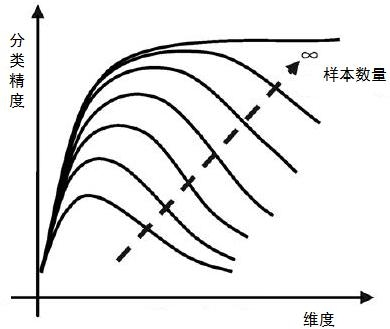
\includegraphics{fig1.jpg}}
    \caption{Example of a figure caption.}
    \label{fig}
\end{figure}


\begin{equation}
    a+b=\gamma\label{eq}
\end{equation}
分隔隔隔隔隔隔隔隔隔隔隔隔隔隔隔隔隔隔隔隔隔隔隔隔隔隔隔隔隔隔隔隔隔隔隔隔隔隔隔隔隔隔隔隔隔隔隔隔隔隔隔隔隔隔隔隔隔隔隔隔隔隔隔隔隔隔隔隔隔隔隔隔隔隔隔隔隔隔隔隔隔隔隔隔隔隔隔隔
\begin{table}[htbp]
    \caption{Table Type Styles}
    \centering
    \begin{tabular}{|c|c|c|c|}
        \hline
        \textbf{Table} & \multicolumn{3}{|c|}{\textbf{Table Column Head}}                                                         \\
        \cline{2-4}
        \textbf{Head}  & \textbf{\textit{Table column subhead}}           & \textbf{\textit{Subhead}} & \textbf{\textit{Subhead}} \\
        \hline
        copy           & 0.12345                   &     中文                     &                           \\
        \hline
        \multicolumn{4}{l}{$^{\mathrm{a}}$Sample of a Table footnote.}
    \end{tabular}
    \label{tab1}
\end{table}

\section{章节二}
引用~\cite{example11}
如图~\ref{fig1}。公式如式~\ref{eq1}。
\begin{figure}[htbp]
    \centerline{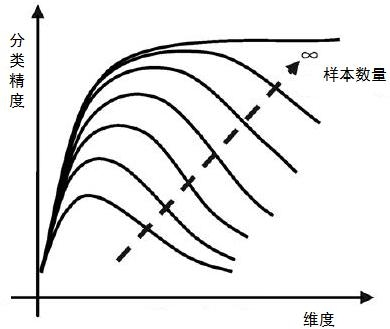
\includegraphics{fig1.jpg}}
    \caption{Example of a figure caption.}
    \label{fig1}
\end{figure}


\begin{equation}
    a+b=\gamma\label{eq1}
\end{equation}
分隔隔隔隔隔隔隔隔隔隔隔隔隔隔隔隔隔隔隔隔隔隔隔隔隔隔隔隔隔隔隔隔隔隔隔隔隔隔隔隔隔隔隔隔隔隔隔隔隔隔隔隔隔隔隔隔隔隔隔隔隔隔隔隔隔隔隔隔隔隔隔隔隔隔隔隔隔隔隔隔隔隔隔隔隔隔隔隔
\begin{table}[htbp]
    \caption{Table Type Styles}
    \centering
    \begin{tabular}{|c|c|c|c|}
        \hline
        \textbf{Table} & \multicolumn{3}{|c|}{\textbf{Table Column Head}}                                                         \\
        \cline{2-4}
        \textbf{Head}  & \textbf{\textit{Table column subhead}}           & \textbf{\textit{Subhead}} & \textbf{\textit{Subhead}} \\
        \hline
        copy           & 0.12345                   &     中文                     &                           \\
        \hline
        \multicolumn{4}{l}{$^{\mathrm{a}}$Sample of a Table footnote.}
    \end{tabular}
    \label{tab2}
\end{table}

\bibliographystyle{gbt7714-2005}
\markright{} % 清除左右页眉
\bibliography{mybib}
\markboth{}{} %清除左右页眉

% \input{thanks.tex}
% \input{myPapers.tex}

\end{document}